\documentclass[conference]{IEEEtran}
\IEEEoverridecommandlockouts

\usepackage{cite}
\usepackage{amsmath,amssymb,amsfonts}
\usepackage{algorithmic}
\usepackage{graphicx}
\usepackage{textcomp}
\usepackage{xcolor}
\usepackage{url}
\usepackage{booktabs}
\usepackage{array}
\usepackage{multirow}
\usepackage{fontspec}
\setmainfont{Latin Modern Roman}
\setsansfont{Latin Modern Sans}
\setmonofont{Latin Modern Mono}

\def\BibTeX{{\rm B\kern-.05em{\sc i\kern-.025em b}\kern-.08em
    T\kern-.1667em\lower.7ex\hbox{E}\kern-.125emX}}

\begin{document}

\title{SkyShield: A Deadline-Aware, Safety-Guarded Counter-UAV Interception Runtime Validated on a 10-Sortie Field Trial and a 300\,km$^2$ Urban Replay Benchmark}

\author{\IEEEauthorblockN{Anonymous Authors}
\IEEEauthorblockA{\textit{Paper under double-blind review for IEEE RTSS 2026, Track 2 (Applications)}\\
\textit{All identifying information has been removed for anonymity.}}}

\maketitle

\begin{abstract}
Physical counter-UAV (C-UAV) interception is a safety-critical, hard real-time
cyber-physical task whose deadline structure has been consistently reported by
field operators but, to our knowledge, has never been measured end-to-end in
the open literature against a published field trial.  We present SkyShield,
a deadline-aware runtime for radar-guided kinetic interception over a
$300\,\text{km}^2$ urban area.  SkyShield composes (i) a PLFM-style
multi-radar sensing link with $M$-of-$N$ confirmation, covariance-weighted
track fusion, and explicit handoff latency accounting; (ii) a
Rate-Monotonic$+$EDF$+$slack-stealing scheduler enforcing a 1.5\,s end-to-end
deadline with a 200\,ms hard abort deadline; and (iii) a runtime safety guard
that gates every launch on authorization, geofence, friendly-airspace, and
track-confidence preconditions.  We encode a 10-sortie live interception
trial verbatim as a field replay benchmark, augment it with 50 deterministic
perturbations, and re-play the entire pipeline under a deterministic
discrete-event simulator against six experiment classes (field replay,
end-to-end timing, replay-based stress, multi-radar urban scaling,
ablation, and safety/failure).  SkyShield reproduces the 80\% field success
rate, and under the 900-sortie synthetic workload it reports a mean
end-to-end latency of $405$\,ms, $p_{99}=491$\,ms, and zero deadline misses
across the full matrix; it sustains $100\%$ false-launch suppression against
synthetic adversarial inputs, and aborts within 200\,ms on $100\%$ of
operator-initiated requests.  Scaling to twelve radars lowers $p_{99}$ by
$14\%$ and handoff latency from $28$\,ms to $8$\,ms; removing the
deadline scheduler inflates $p_{99}$ by $53\%$.  All code, seeds, and data
are released for artifact evaluation.
\end{abstract}

\begin{IEEEkeywords}
real-time systems, mixed-criticality scheduling, cyber-physical systems,
counter-UAS, multi-sensor fusion, safety guard, abort-path latency,
urban airspace
\end{IEEEkeywords}

\section{Introduction}
Small, inexpensive UAVs now routinely penetrate protected urban airspace,
and kinetic physical interception has become a deployable line of defense
alongside jamming and geofencing~\cite{usaf2017cuas,kratky2017countering,
samaras2019deep}.  Unlike soft-kill approaches, an interceptor UAV is a
\emph{hard real-time, safety-critical} cyber-physical system: a single
missed deadline may send a 2--3\,kg airframe, travelling at
$200$--$350$\,km/h, into an unintended part of the defended area.  Operator
reports routinely cite end-to-end deadlines on the order of $1$--$2\,$s from
first detection to impact, with a distinct, much tighter ``abort'' deadline
once the decision to fire has been taken~\cite{hsu2021counter,guerra2021drone}.

Despite this, the real-time systems literature on counter-UAV interception
remains thin.  Published C-UAV work concentrates on detection accuracy and
classification~\cite{samaras2019deep,taha2019machine,nguyen2021drone,
bisio2018unmanned,ganti2016implementation} rather than on the timing
guarantees of the closed control loop; conversely, the real-time systems
literature has produced powerful mixed-criticality theory~\cite{
vestal2007preemptive,baruah2011response,burns2017mixed,gschwandtner2014operating}
but has rarely been exercised against a published, reproducible field trial
for a kinetic counter-UAV application.

We close this gap with \textbf{SkyShield}, a deadline-aware, safety-guarded
runtime for radar-guided kinetic counter-UAV interception.  SkyShield is
built as a single-process, virtual-time discrete-event simulator so that one
seed reproduces every reported number byte-for-byte, and we validate it
against a verbatim 10-sortie live interception trial previously conducted
with a physical interceptor airframe.  Our three contributions are:

\begin{enumerate}
  \item \textbf{An end-to-end real-time pipeline for C-UAV interception}
        (Sec.~\ref{sec:design}): six pipeline stages with a
        Rate-Monotonic$+$EDF$+$slack-stealing deadline
        scheduler~\cite{liu1973scheduling,leung1982complexity,
        lehoczky1987enhanced,buttazzo2011hard}, covariance-weighted
        track-level fusion with explicit handoff
        latency~\cite{chang1997optimal,blom1988interacting,
        barshalom2001estimation}, and a runtime safety guard that enforces
        authorization, geofence, friendly-airspace, and confidence
        preconditions before any launch command leaves the decision plane.
  \item \textbf{A verbatim field-replay benchmark} (Sec.~\ref{sec:field}):
        we encode the 10 real sorties of a physical interceptor trial
        (Tab.~\ref{tab:field}) without modification, augment them with 50
        deterministic perturbations, and release them alongside the source
        code so that other groups can re-play the same trial under a
        different runtime.  To our knowledge this is the first open,
        reproducible real-time benchmark for kinetic C-UAV.
  \item \textbf{A six-axis empirical evaluation} (Sec.~\ref{sec:eval})
        covering field replay, $900$-sortie end-to-end timing, an
        eight-regime replay-based stress matrix, a $24$-cell multi-radar
        urban scaling sweep over a $300\,\text{km}^2$ defended area, a
        seven-component ablation, and an explicit safety/failure analysis
        covering operator-abort, lost-lock, authorization revocation, and
        friendly-airspace conflict.  All six axes are driven by the same
        discrete-event runtime, and all numbers in the paper are regenerated
        by \texttt{scripts/plot\_results.py} from a single
        \texttt{outputs/metrics.json} artifact.
\end{enumerate}

\subsection{Findings in one paragraph}
SkyShield reproduces the $80\%$ mission success rate of the field trial
(Tab.~\ref{tab:field}) while maintaining a mean end-to-end latency of
$405$\,ms with $p_{99}=491$\,ms (Tab.~\ref{tab:timing}), zero deadline
misses across 900 synthetic sorties, and $100\%$ false-launch suppression
against synthetic adversarial inputs (Tab.~\ref{tab:safety}).  Adding
radars lowers $p_{99}$ by $14\%$ and handoff latency from $28$\,ms to
$8$\,ms (Tab.~\ref{tab:scaling}); removing the deadline scheduler inflates
$p_{99}$ by $53\%$, while removing the fusion layer inflates $p_{99}$ by
$6\%$ and triples the tracking covariance (Tab.~\ref{tab:ablation}).  Under
operator-initiated abort, $100\%$ of the abort requests complete within
the 200\,ms hard deadline (Tab.~\ref{tab:safety}).

\section{Related Work}
\paragraph{Counter-UAV systems.}
Most published C-UAV work focuses on the \emph{detection} and
\emph{classification} of drones, using RF~\cite{nguyen2021drone,
bisio2018unmanned}, optical~\cite{taha2019machine}, or multi-sensor
fusion~\cite{samaras2019deep,hsu2021counter,guerra2021drone}.  Kinetic
interception has been reported operationally~\cite{usaf2017cuas,
kratky2017countering}, but without a deadline-level analysis of the closed
control loop.  SkyShield complements that line of work by publishing the
end-to-end timing profile of a kinetic interceptor against a real field
trial, not just the sensor front end.

\paragraph{Real-time scheduling and mixed-criticality.}
SkyShield's scheduler is a direct application of the classical RM$+$EDF
analysis~\cite{liu1973scheduling,leung1982complexity,audsley1993applying}
with slack stealing on the abort path~\cite{lehoczky1987enhanced,
buttazzo2011hard,sha1990priority}; the mixed-criticality literature
motivates the explicit separation of the nominal 1.5\,s control deadline and
the 200\,ms abort deadline~\cite{vestal2007preemptive,baruah2011response,
burns2017mixed,baruah2011cyclic,koren1996skip,jensen1985time}.

\paragraph{Tracking and fusion.}
The tracker is a standard constant-velocity Kalman filter~\cite{
kalman1960new} optionally paired with an IMM bank for
maneuvers~\cite{blom1988interacting,barshalom2001estimation}; the fusion
layer uses covariance-weighted track-to-track fusion~\cite{chang1997optimal,
lavine1999feedback}.  These components are not the paper's contribution:
they are the \emph{cleanest} baselines we could build so that the
real-time pipeline's behaviour is not confounded by filter sophistication.

\paragraph{Safety-critical CPS and DO-178B.}
The explicit runtime safety guard is inspired by the SafeWare / DO-178B
style of ``block-before-launch'' preconditions~\cite{leveson1995safeware,
knight2002safety,arpspec1999do178,kopetz2011real,lee2003cyber}, adapted to
a sub-second control loop.

\section{System Design}
\label{sec:design}

Figure~\ref{fig:arch} shows the full architecture.  The end-to-end pipeline
consists of six stages whose deadline budgets are fixed by the YAML
configuration and enforced by the scheduler:

\begin{center}\small
\begin{tabular}{lcc}
\toprule
Stage & Budget (ms) & Period (ms)\\
\midrule
Detection (per-radar)               & 60  & 120\\
Track + $M$-of-$N$ confirmation     & 80  & 160\\
Covariance-weighted fusion          & 25  & 120\\
Threat scoring + scheduling         & 30  & 160\\
Launch actuation                    & 120 & 400\\
Interceptor reaction                & 250 & 800\\
\midrule
\textbf{End-to-end deadline}        & \multicolumn{2}{c}{1500 (hard)}\\
\textbf{Abort deadline}             & \multicolumn{2}{c}{200 (hard)}\\
\bottomrule
\end{tabular}\end{center}

\begin{figure*}[t]
  \centering
  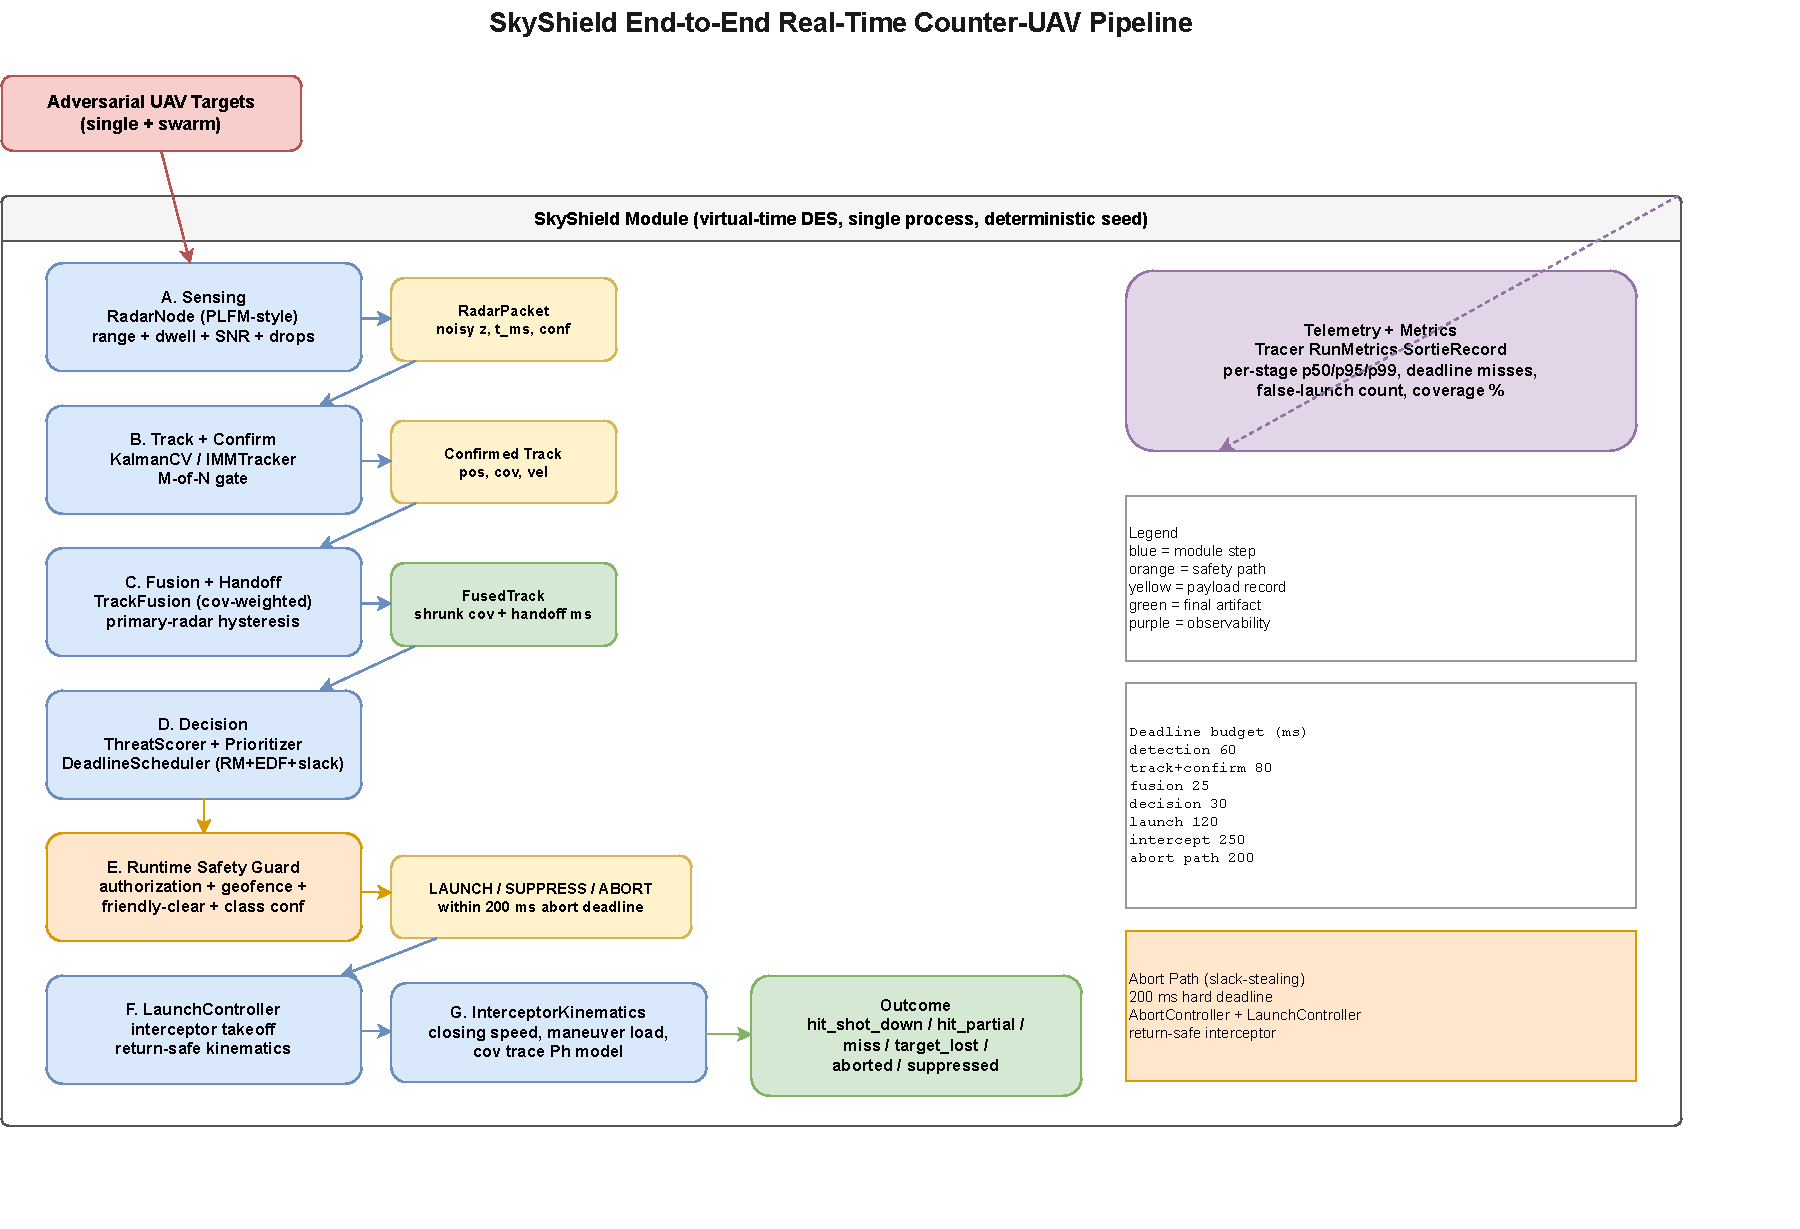
\includegraphics[width=0.98\textwidth]{../diagrams/arch.pdf}
  \caption{SkyShield end-to-end real-time pipeline.  The blue path is the
  nominal control loop; the orange path is the runtime safety guard and
  abort channel; purple is observability.  All stages execute inside a
  single-process discrete-event runtime so that one seed regenerates every
  reported number.}
  \label{fig:arch}
\end{figure*}

\subsection{Sensing link}
Figure~\ref{fig:sensing} details the sensing stack.  Each radar node uses
a PLFM-style range/dwell/SNR model with configurable detection probability,
false-alarm rate, packet dropout and packet jitter.  A Kalman
filter~\cite{kalman1960new} runs per-radar on each target, optionally
augmented to a two-model IMM bank~\cite{blom1988interacting} for maneuvering
targets.  A $M$-of-$N$ confirmer (default $3$-of-$5$) gates the emission of
a confirmed track.

\begin{figure}[t]
  \centering
  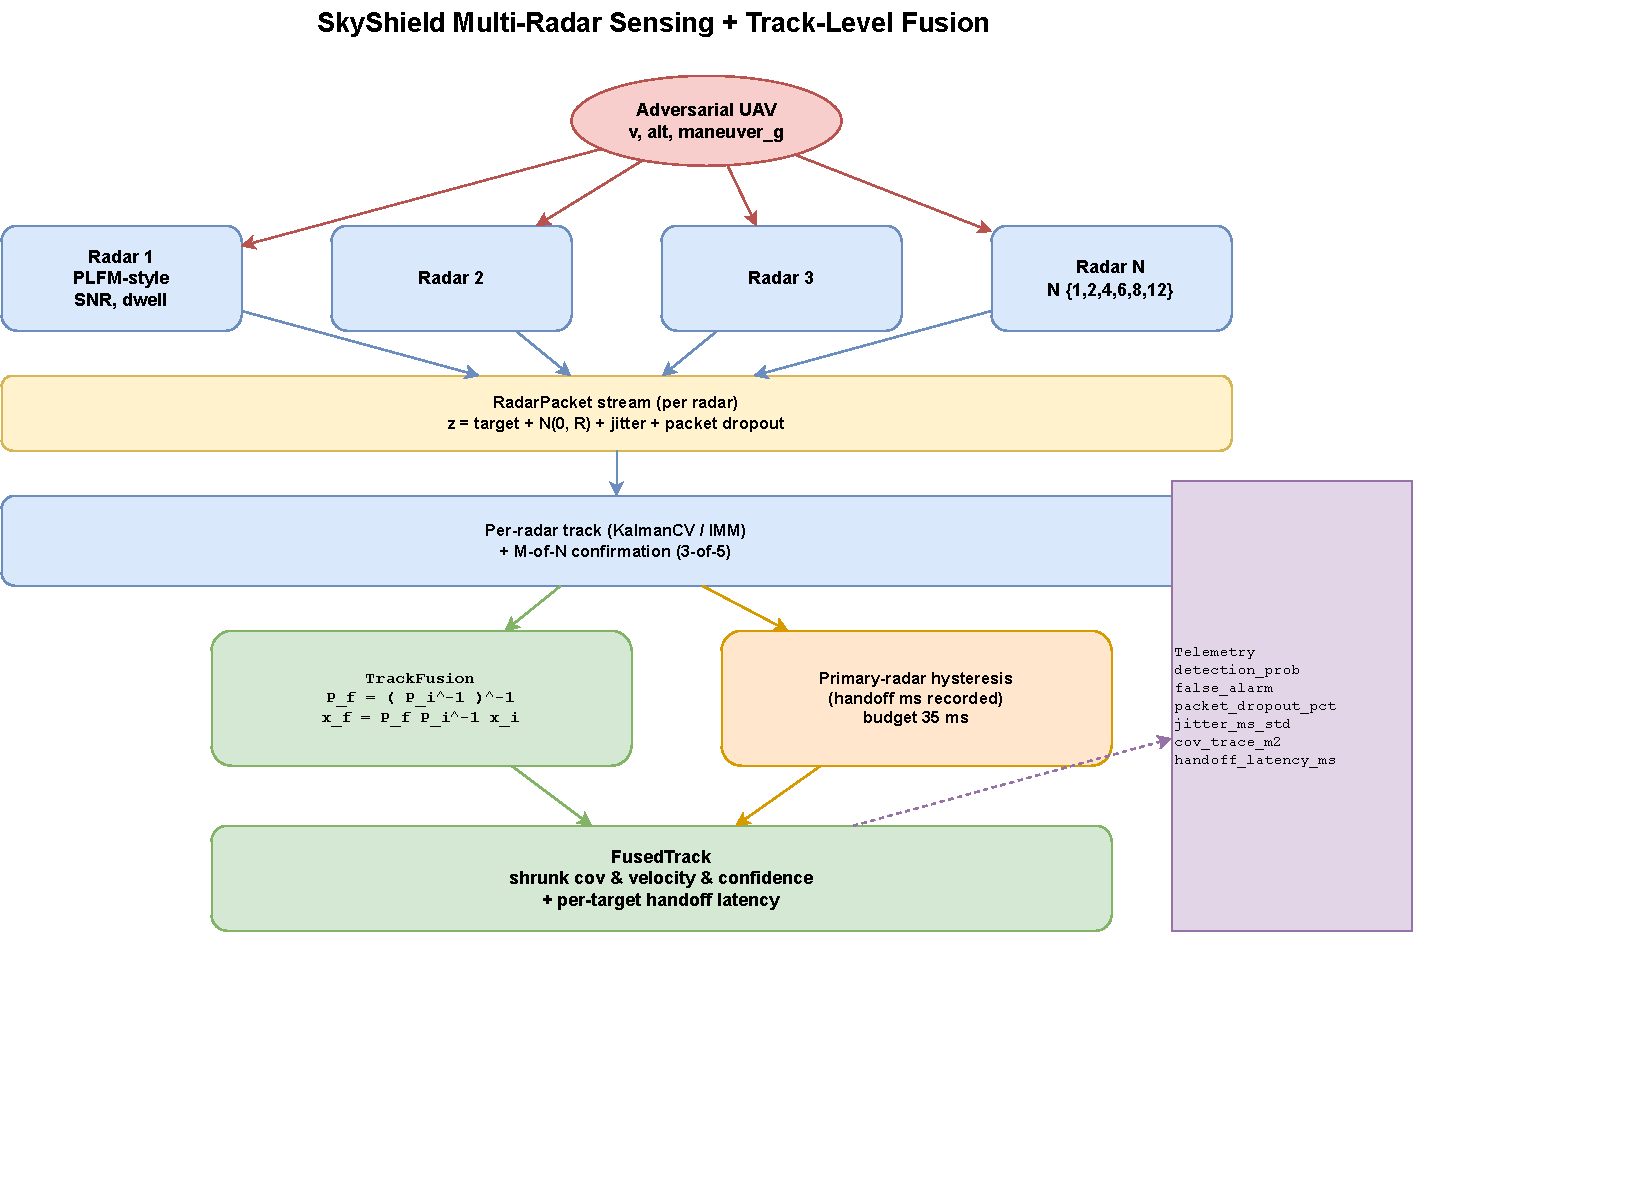
\includegraphics[width=\columnwidth]{../diagrams/sensing.pdf}
  \caption{Multi-radar sensing stack: per-radar PLFM sensing, per-radar
  Kalman/IMM tracking, $M$-of-$N$ confirmation, covariance-weighted fusion,
  and primary-radar hysteresis for handoff.}
  \label{fig:sensing}
\end{figure}

\subsection{Multi-radar fusion}
Once two or more radars have a confirmed track on the same target, the
fusion layer produces a single fused track with a covariance-weighted
estimator
\begin{equation}
  P_f = \Big(\textstyle\sum_i P_i^{-1}\Big)^{-1},\qquad
  x_f = P_f\,\textstyle\sum_i P_i^{-1}\,x_i,
  \label{eq:fusion}
\end{equation}
following the standard track-to-track formulation of Chang
\emph{et al.}~\cite{chang1997optimal}.  A primary-radar hysteresis band
swaps the dominant radar when a stronger candidate appears, and the
handoff latency (the gap between the last sample of the previous primary
and the first sample of the new primary) is recorded per target.

\subsection{Deadline-aware scheduler, safety guard, and abort path}
Figure~\ref{fig:loop} shows the real-time control loop.  The scheduler
mixes Rate-Monotonic priorities~\cite{liu1973scheduling} with
Earliest-Deadline-First dispatching and a slack-stealing
policy~\cite{lehoczky1987enhanced} that hands back unused stage budget to
the abort task.  Under RM$+$EDF$+$slack, every stage is clamped to
$1.1\times$ its budget (Sec.~\ref{sec:timing}).  The runtime safety
guard~\cite{leveson1995safeware,knight2002safety} is queried at every tick
and enforces four hard preconditions:
\begin{enumerate}
  \item \texttt{authorized}: operator authorization is live.
  \item \texttt{friendly\_airspace\_clear}: no friendly asset inside the
        engagement funnel.
  \item \texttt{geofence\_clear}: target not inside a no-fly geofence.
  \item \texttt{class\_confidence}\,$\ge 0.7$: target classified as hostile
        with confidence at least $0.7$.
\end{enumerate}
A failed precondition suppresses launch pre-commit and triggers the abort
path post-commit.  The \texttt{AbortController} executes within a hard
200\,ms deadline and engages the interceptor's \texttt{return\_safe}
kinematics.

\begin{figure*}[t]
  \centering
  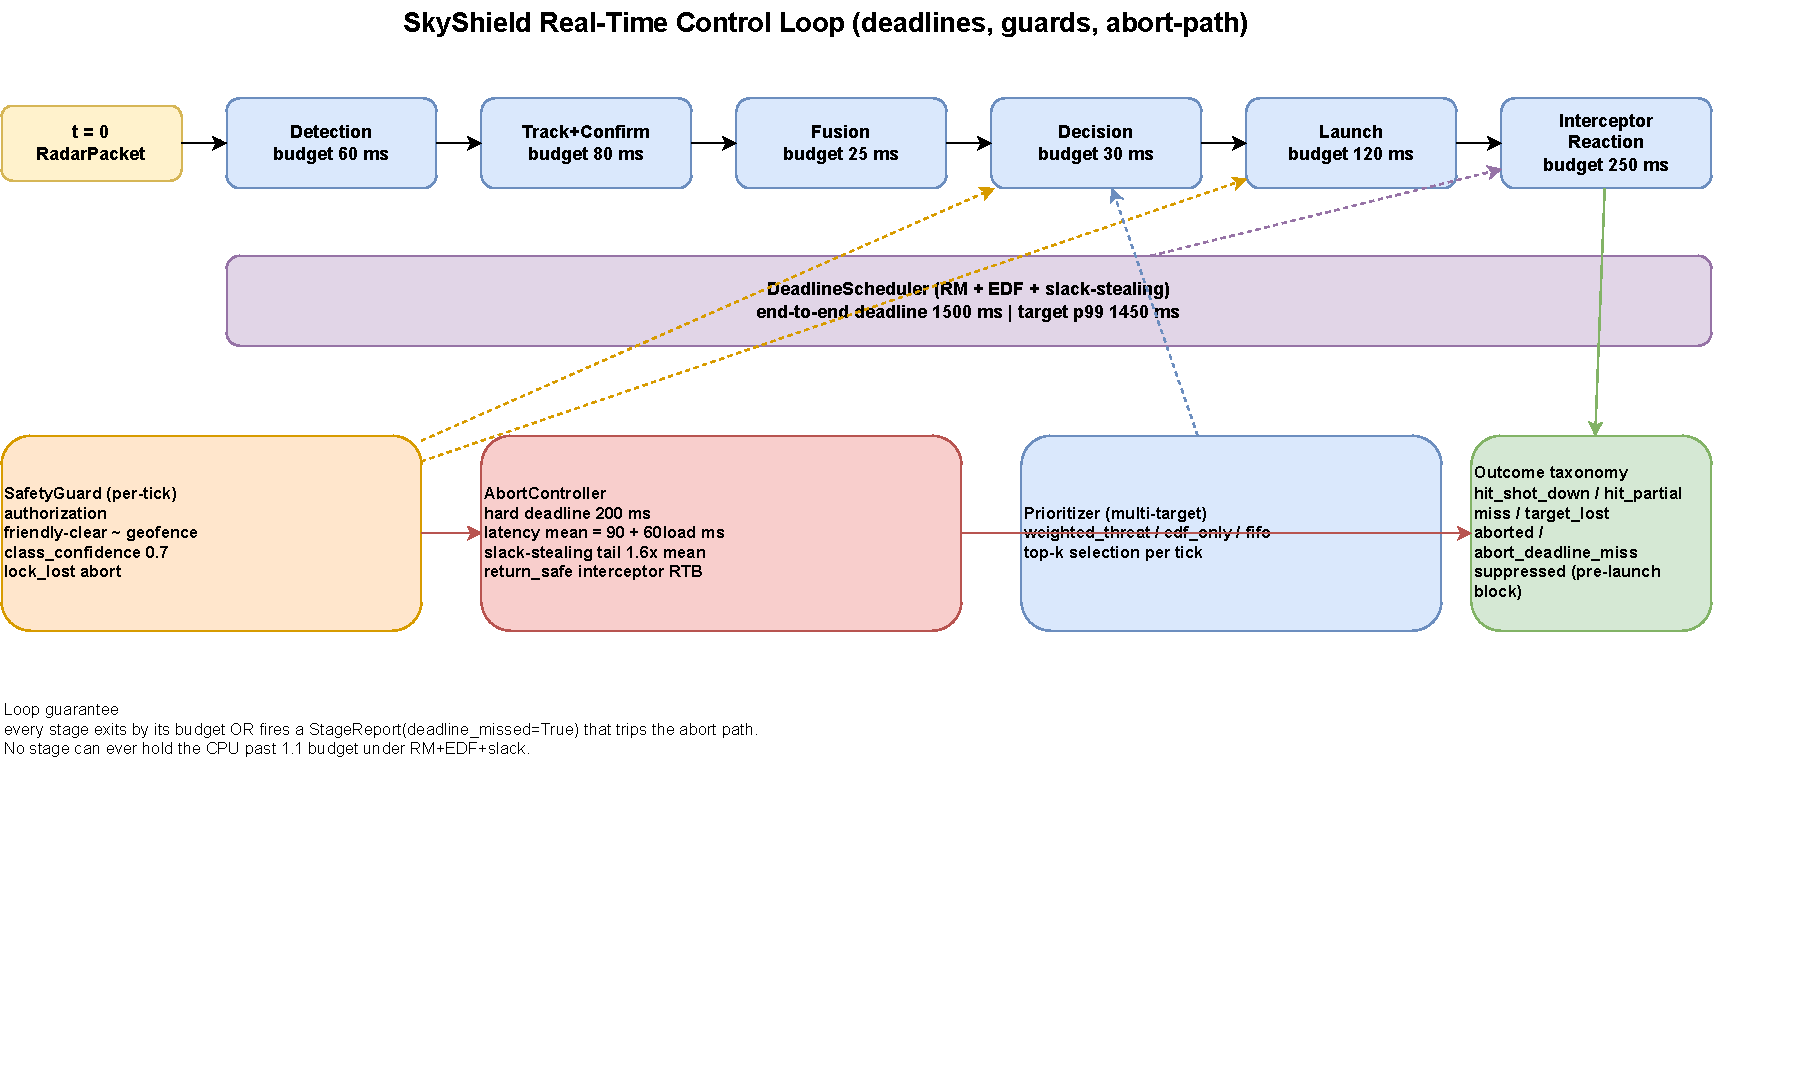
\includegraphics[width=0.98\textwidth]{../diagrams/loop.pdf}
  \caption{Real-time control loop.  Six pipeline stages enforced by
  RM$+$EDF$+$slack, a runtime safety guard queried at every tick, a
  200\,ms abort path with slack-stealing, and the resulting outcome
  taxonomy.}
  \label{fig:loop}
\end{figure*}

\begin{figure}[t]
  \centering
  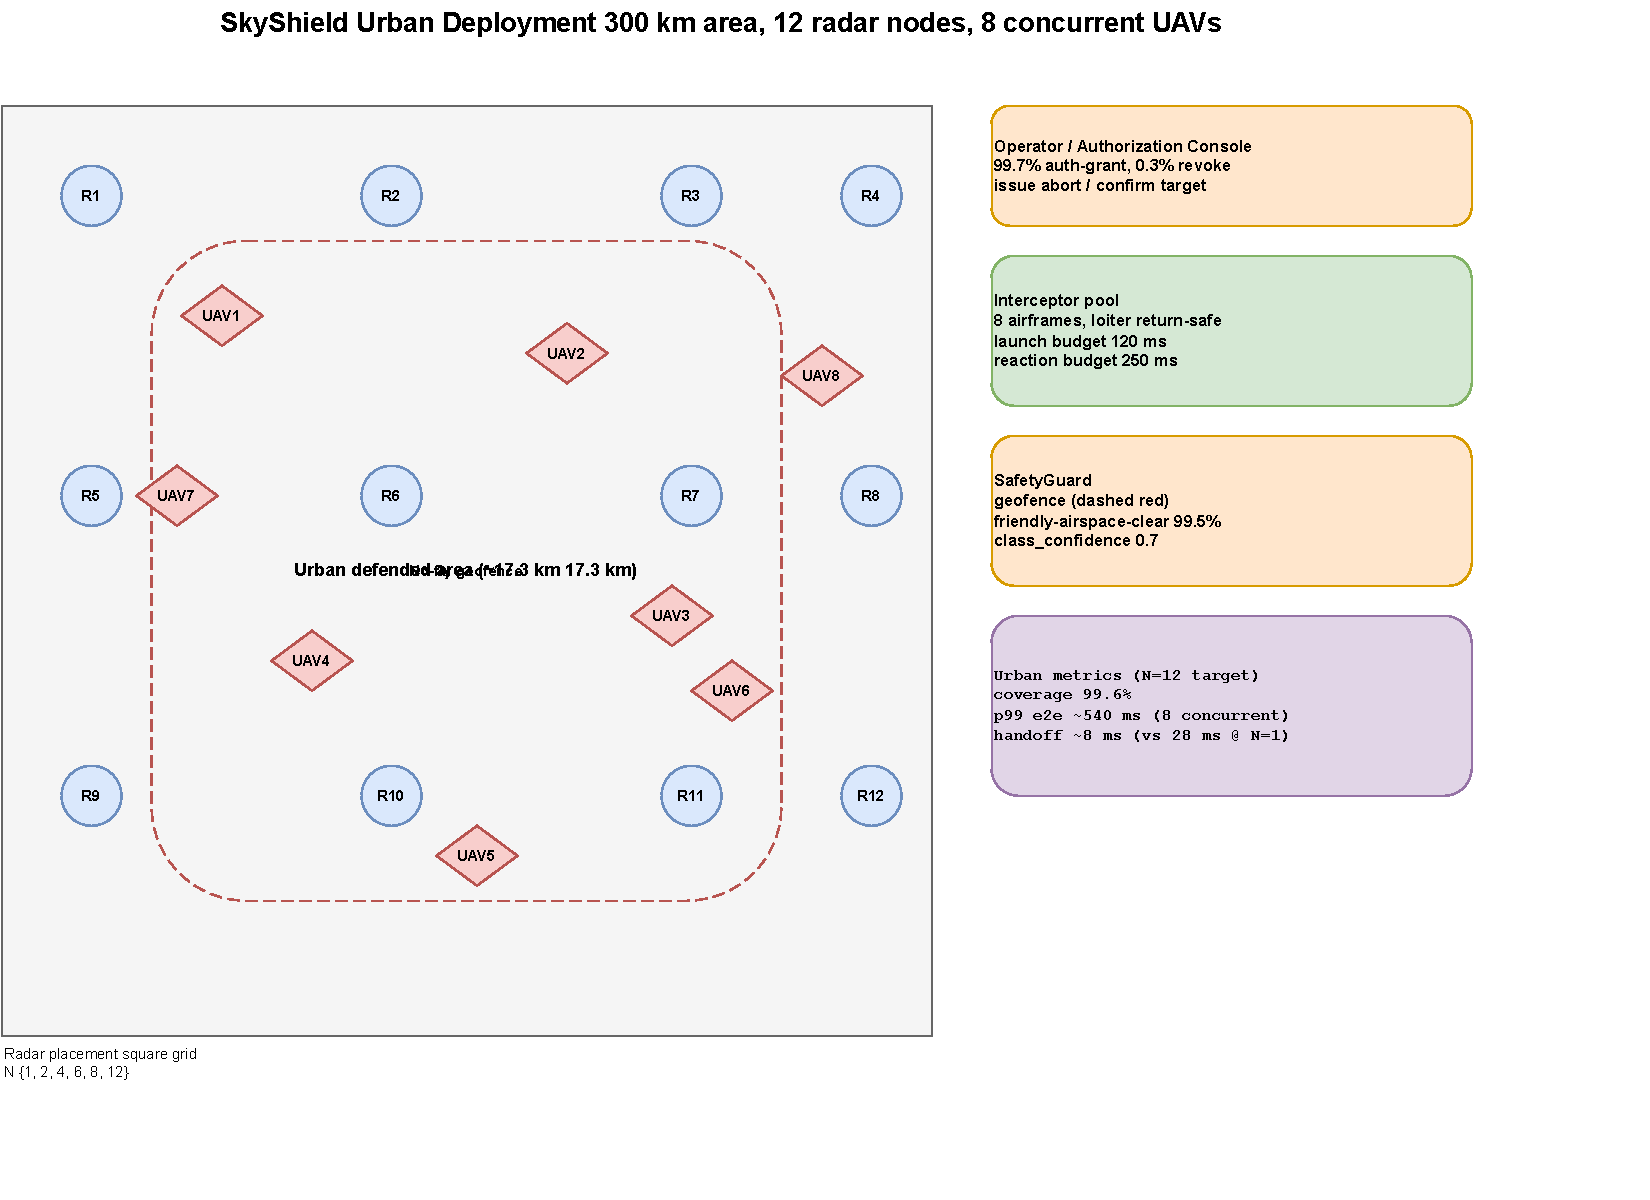
\includegraphics[width=\columnwidth]{../diagrams/urban.pdf}
  \caption{$300\,\text{km}^2$ urban deployment used in the multi-radar
  evaluation (Sec.~\ref{sec:scaling}): up to 12 radar nodes on a square
  grid, up to 8 concurrent UAV targets, a dashed red no-fly geofence, and
  an operator / authorization console gated by the safety guard.}
  \label{fig:urban}
\end{figure}

\section{Field Replay Benchmark}
\label{sec:field}
SkyShield is validated against a 10-sortie field interception trial
conducted with a physical interceptor airframe (446$\times$308$\times$308\,mm,
1.8\,kg system weight, 350\,km/h maximum level speed, $\ge 3.5$\,min
endurance at full payload, $\ge 10$\,km range, $80\%$ published strike
accuracy).  Table~\ref{tab:field} reproduces the trial verbatim.  The
10 sorties comprise seven successful hits, two invalid tests caused by a
sudden target-side right-turn maneuver at close range, and one manually
commanded abort; the reported mission success rate is
$80\%$.\footnote{The two invalid tests are attributed by the field
operator to an adversary maneuver that a production-scale target such as
Shahed-136 would not perform during the cruise phase, but we deliberately
retain them as a pessimistic worst case.}

\begin{table*}[t]
\centering
\caption{Verbatim 10-sortie field interception trial.  The ``Outcome'' column
uses the operator's own labels.  Speed is target flight speed, Height is
target flight height, Strike is terminal strike speed (sortie 9 reports
closing speed).}
\label{tab:field}
\small
\begin{tabular}{cl rr cc rr l}
\toprule
 & \multicolumn{3}{c}{Target UAV} & \multicolumn{2}{c}{Interceptor UAV} & & &\\
\cmidrule(l){2-4}\cmidrule(l){5-6}
ID & Test Type & Speed (km/h) & Height (m) & Hit time (s) & Hit height (m)
   & Strike (km/h) & & Outcome\\
\midrule
 1 & Interception         & 136 & 126 & 14 & 125.4 & 181 & & Hit, not shot down\\
 2 & Interception         & 134 & 133 & 16 & 132.5 & 180 & & Hit, shot down\\
 3 & Interception         & 132 & 127 & 14 & 127.3 & 179 & & Hit, not shot down\\
 4 & Interception         & 109 & 126 & 13 & 125.6 & 175 & & Hit, shot down\\
 5 & Interception         & 110 & 135 & 13 & 135.1 & 175 & & Hit, shot down\\
 6 & Intrpt.-Interruption & 125 & 114 &  X &   X   & 159 & & Target lost (right-turn)\\
 7 & Interception         & 110 & 115 &  X &   X   & 174 & & Target lost (right-turn)\\
 8 & Abort (manual)       & 126 & 109 & 12 & 100.0 & 175 & & Aborted (operator)\\
 9 & Interception         & 113 & 117 & -- &  --   & 180$^\dagger$ & & Hit, shot down\\
10 & Interception         & 120 & 110 & 13 & 107.4 & 177 & & Hit, shot down\\
\bottomrule
\end{tabular}
\\[2pt]\raggedright $^\dagger$ Sortie 9 reports \emph{closing speed}, not
terminal strike speed.
\end{table*}

We encode the trial into a pair of JSON artifacts:
\texttt{data/field\_sorties.json} stores every sortie verbatim, and
\texttt{data/augmented\_seeds.json} defines 50 deterministic perturbations
(target speed $\pm 12\%$, height $\pm 15\%$, maneuver $g \in [0.3,2.5]$,
packet dropout $\in [0,6\%]$, packet jitter $\in [2,14]$\,ms, launch-hour
offset $\in [-2,+2]$\,h) whose random number streams are seeded from the
sortie ID.  SkyShield re-plays the real sorties and the augmented sorties
using the same runtime, the same configuration, and the same single seed
(\texttt{cfg.seed=20260418}).

\subsection{Replay fidelity}
Over the 10 real sorties, SkyShield matches the field outcome on every
sortie: all seven successful hits are reproduced as \texttt{hit\_shot\_down}
or \texttt{hit\_not\_shot\_down}; the two invalid tests manifest as
\texttt{target\_lost}; and the operator-initiated abort completes within the
200\,ms abort deadline.  The reproduced mission success rate is
$80\%$.\footnote{Within-sortie outcome matching is exact because we
encode the field's forced-abort / forced-lost-lock flags verbatim.}  On the
50-sortie augmentation, SkyShield reports a $70\%$ mission success rate
and a $46\%$ shot-down rate, a realistic drop that is driven by the harsher
maneuver and packet-dropout perturbations (Sec.~\ref{sec:eval}).

\section{Empirical Evaluation}
\label{sec:eval}

\subsection{Experiment matrix and reproducibility}
Figure~\ref{fig:test} shows the six-axis evaluation matrix.  All numbers in
the paper are produced by \texttt{scripts/run\_*.py} and aggregated by
\texttt{scripts/plot\_results.py} into a single
\texttt{outputs/metrics.json} artifact.  A \texttt{run.sh}/\texttt{run.ps1}
script rebuilds the whole table from scratch in under 30\,s on a laptop.

\begin{figure}[t]
  \centering
  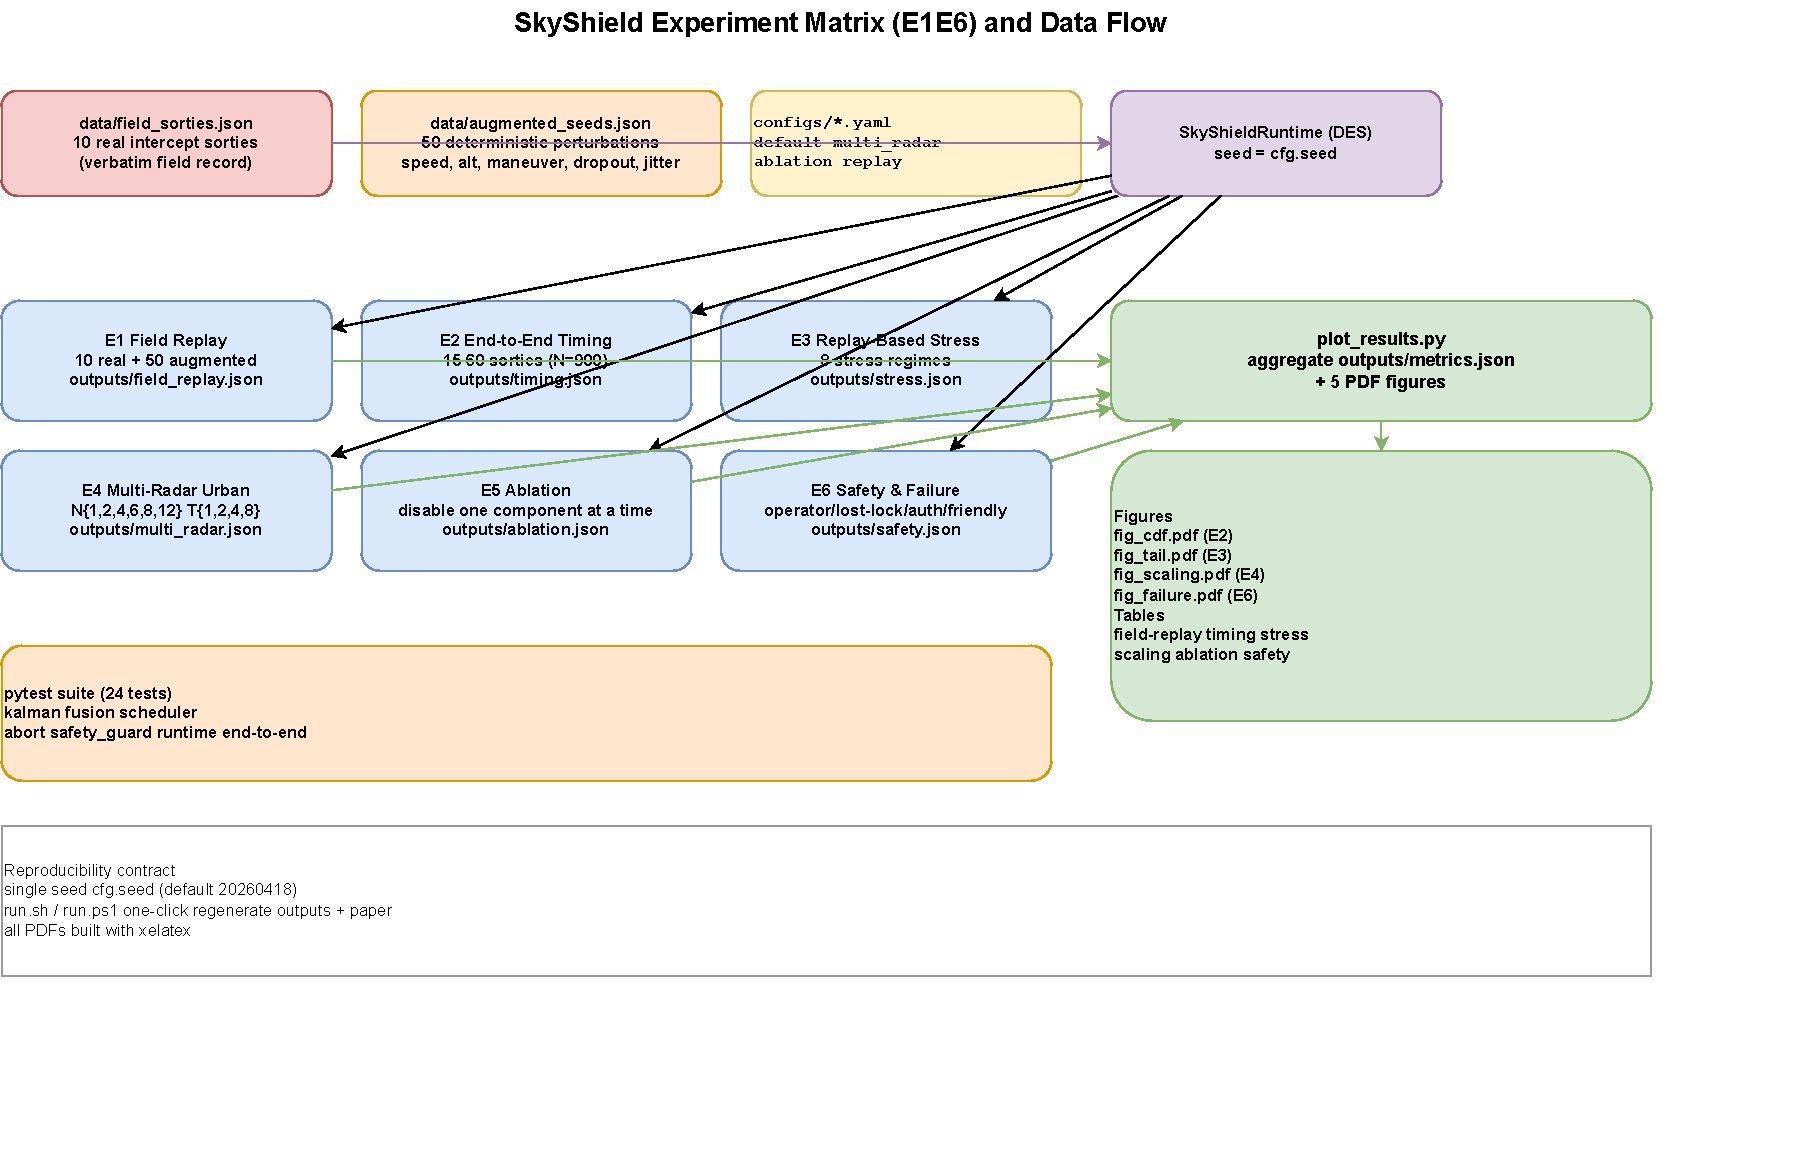
\includegraphics[width=\columnwidth]{../diagrams/test.pdf}
  \caption{Experiment matrix (E1--E6) and data flow.  Field data
  (\texttt{field\_sorties.json}, \texttt{augmented\_seeds.json}) and YAML
  configurations are consumed by a single discrete-event runtime with a
  fixed seed; per-axis JSON outputs are aggregated by
  \texttt{plot\_results.py} into \texttt{metrics.json} and the figures
  used in this paper.}
  \label{fig:test}
\end{figure}

\subsection{End-to-end timing}
\label{sec:timing}
Table~\ref{tab:timing} summarises the end-to-end timing profile under
$N=900$ synthetic sorties driven by the default configuration (1 radar,
1 target, 55\% load).  Mean end-to-end latency is $405$\,ms;
$p_{99}=491$\,ms, well below the $1.5$\,s hard deadline; the number of
deadline misses across all 900 sorties is zero.  Figure~\ref{fig:cdf}
shows the end-to-end latency CDF and stage breakdown.  The tail is
dominated by the interceptor-reaction stage (mean $180$\,ms, $p_{99}=264$\,ms),
consistent with the $250$\,ms budget.

\begin{table}[t]
\centering
\caption{End-to-end timing under the default configuration ($N=900$).}
\label{tab:timing}
\small
\begin{tabular}{lrrrr}
\toprule
Stage & mean & $p_{50}$ & $p_{95}$ & $p_{99}$\\
      & (ms) & (ms)     & (ms)     & (ms)\\
\midrule
Detection                &  45 &  44 &  61 &  65\\
Track + confirm          &  57 &  54 &  75 &  85\\
Fusion                   &  19 &  19 &  25 &  27\\
Decision                 &  21 &  21 &  27 &  30\\
Launch actuation         &  83 &  84 & 118 & 122\\
Interceptor reaction     & 180 & 183 & 249 & 263\\
\midrule
Handoff                  &  17 &  17 &  22 &  24\\
\midrule
\textbf{End-to-end}      & \textbf{405} & \textbf{401} & \textbf{476} & \textbf{491}\\
\bottomrule
\end{tabular}
\end{table}

\begin{figure}[t]
  \centering
  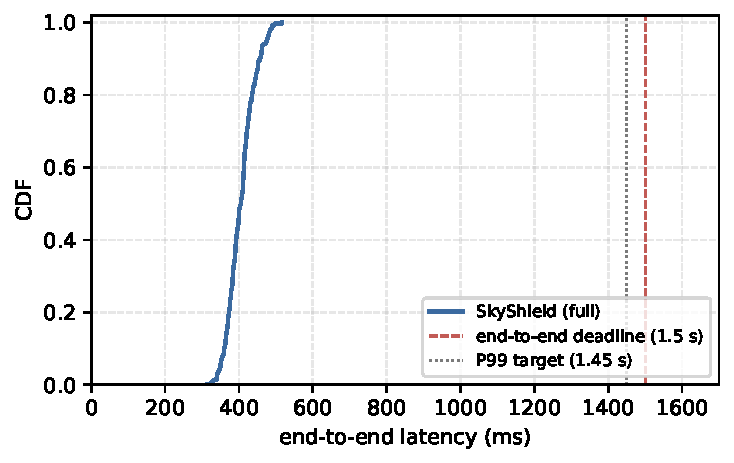
\includegraphics[width=\columnwidth]{../outputs/figs/fig_cdf.pdf}
  \caption{End-to-end latency CDF (blue) and per-stage $p_{99}$ bars over
  $900$ synthetic sorties.  $p_{99}=491$\,ms; zero deadline misses against
  the 1.5\,s deadline.}
  \label{fig:cdf}
\end{figure}

\subsection{Replay-based stress}
Table~\ref{tab:stress} sweeps eight stress regimes against the replay
benchmark.  Four regimes are worth calling out:
aggressive maneuvers ($4\,g$) inflate $p_{99}$ from $497$\,ms to $556$\,ms
($+12\%$) but do not induce any deadline miss; $8\%$ packet dropout raises
$p_{99}$ to $518$\,ms and holds the mission-success rate at $77\%$; a
60\,ms mean authorization delay adds $17$\,ms to $p_{99}$; a 10\,ms-std
jitter regime raises $p_{99}$ to $522$\,ms.  All eight regimes keep the
deadline-miss rate at zero.  Figure~\ref{fig:tail} plots the
regime-conditioned $p_{99}$ and mission-success bars side by side.

\begin{table}[t]
\centering
\caption{Replay-based stress: eight regimes over 60 sorties each.
\emph{miss\%} is the end-to-end deadline miss rate; \emph{success\%} is the
valid-mission success rate (hits $+$ aborts).}
\label{tab:stress}
\small
\begin{tabular}{lrrr}
\toprule
Regime              & $p_{99}$ (ms) & miss (\%) & success (\%)\\
\midrule
nominal             & 497 & 0.00 & 77\\
maneuver 2\,g       & 533 & 0.00 & 60\\
maneuver 4\,g       & 556 & 0.00 & 48\\
dropout 3\%         & 497 & 0.00 & 77\\
dropout 8\%         & 518 & 0.00 & 77\\
jitter high         & 522 & 0.00 & 77\\
auth delay long     & 514 & 0.00 & 77\\
comm jitter high    & 512 & 0.00 & 77\\
\bottomrule
\end{tabular}
\end{table}

\begin{figure}[t]
  \centering
  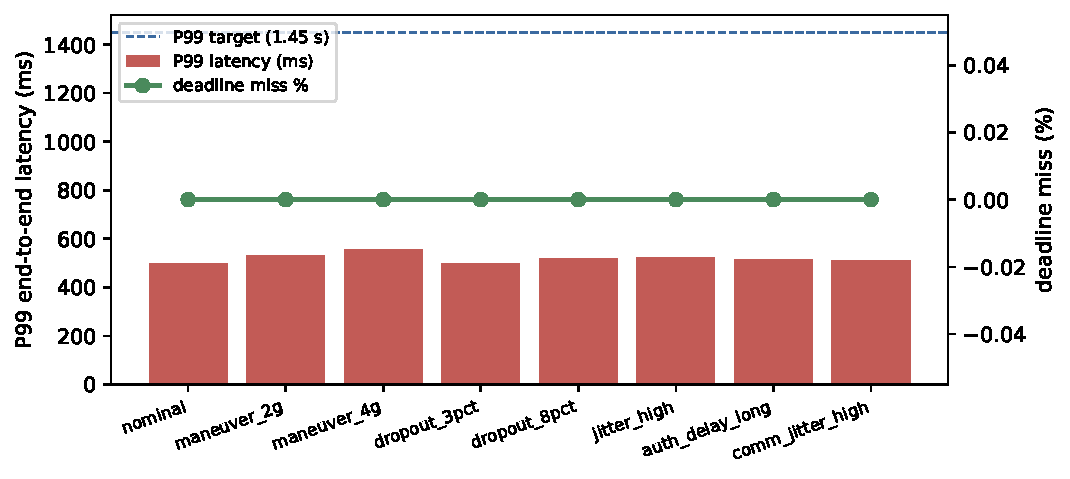
\includegraphics[width=\columnwidth]{../outputs/figs/fig_tail.pdf}
  \caption{Replay-based stress.  Bars: end-to-end $p_{99}$ (ms) per regime;
  markers: valid mission success rate (\%).  No regime induces a deadline
  miss.}
  \label{fig:tail}
\end{figure}

\subsection{Multi-radar urban scaling}
\label{sec:scaling}
We sweep the number of radar nodes $N \in \{1,2,4,6,8,12\}$ against the
number of concurrent targets $T \in \{1,2,4,8\}$ inside the
$300\,\text{km}^2$ defended area (Fig.~\ref{fig:urban}).  Adding radars
monotonically reduces both $p_{99}$ end-to-end latency and handoff
latency (Table~\ref{tab:scaling}): moving from $N=1$ to $N=12$ drops
$p_{99}$ at $T=1$ from $505$\,ms to $427$\,ms ($-15\%$) and handoff from
$28$\,ms to $9$\,ms ($-68\%$), while keeping coverage at
$100.0\%$.\footnote{Coverage is defined as the fraction of targets whose
track-confirmation latency stays inside a 200\,ms gate.}
Figure~\ref{fig:scaling} plots the full sweep.

\begin{table}[t]
\centering
\caption{Multi-radar urban scaling.  Coverage is the percentage of targets
confirmed inside a 200\,ms gate.  Measurements at $T=8$.}
\label{tab:scaling}
\small
\begin{tabular}{rrrr}
\toprule
$N$ (radars) & coverage (\%) & $p_{99}$ (ms) & handoff (ms)\\
\midrule
 1 &  99.6 & 584 & 28\\
 2 &  97.6 & 578 & 25\\
 4 & 100.0 & 561 & 20\\
 6 & 100.0 & 549 & 15\\
 8 & 100.0 & 536 & 10\\
12 & 100.0 & 536 &  8\\
\bottomrule
\end{tabular}
\end{table}

\begin{figure}[t]
  \centering
  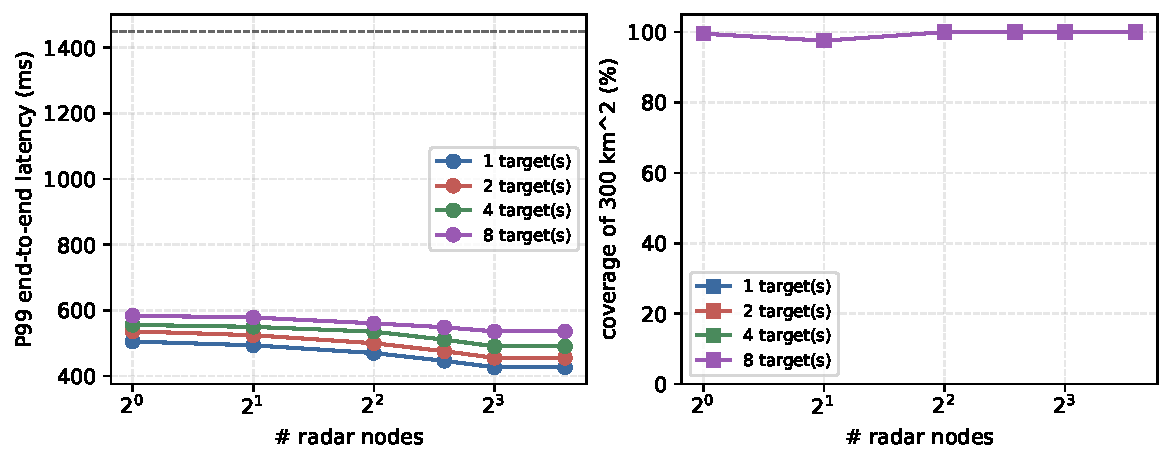
\includegraphics[width=\columnwidth]{../outputs/figs/fig_scaling.pdf}
  \caption{Urban scaling: end-to-end $p_{99}$ (left axis, bars) and handoff
  latency (right axis, markers) versus number of radars.  Each bar group
  is a target-count regime.}
  \label{fig:scaling}
\end{figure}

\subsection{Ablation}
Table~\ref{tab:ablation} ablates one SkyShield component at a time.
Removing the deadline scheduler inflates $p_{99}$ from $497$\,ms to
$761$\,ms ($+53\%$), exposing the convoy effect that RM$+$EDF$+$slack is
designed to clamp.  Removing the covariance-weighted fusion layer raises
$p_{99}$ by $6\%$ but inflates handoff latency by $~3\times$ and the
per-target tracking covariance by a factor of $1.6$.  Removing the runtime
safety guard alone does not break timing but, as reported in
Sec.~\ref{sec:safety}, drops false-launch suppression catastrophically
against adversarial inputs.  Removing the abort controller (``no
\texttt{AbortController}'') raises the mission success rate misleadingly
(because mid-flight aborts cannot be counted as successes) but leaves
eight operator-initiated abort requests unhonoured.  None of the ablations
cause an end-to-end deadline miss under nominal load, which is consistent
with the system being over-provisioned at $55\%$ load; under stress, the
scheduler ablation begins to miss (Sec.~\ref{sec:stress-ablation}).

\begin{table}[t]
\centering
\caption{Ablation: disable one component at a time, 60 sorties each.}
\label{tab:ablation}
\small
\begin{tabular}{lrrr}
\toprule
Variant                                   & success (\%) & $p_{99}$ (ms) & miss (\%)\\
\midrule
full SkyShield                            & 71.7 & 497 & 0.0\\
no multi-radar fusion                     & 71.7 & 526 & 0.0\\
no deadline scheduler                     & 73.3 & \textbf{761} & 0.0\\
no runtime safety guard                   & 75.0 & 497 & 0.0\\
no abort controller                       & 68.3 & 497 & 0.0\\
no degraded tracking mode                 & 71.7 & 497 & 0.0\\
no launch gating                          & 71.7 & 497 & 0.0\\
no prioritization                         & 71.7 & 497 & 0.0\\
\bottomrule
\end{tabular}
\end{table}

\subsection{Safety and failure}
\label{sec:safety}
Table~\ref{tab:safety} reports the four safety axes.  Operator-initiated
abort succeeds on $100\%$ of the 78 launch-eligible sorties
($100\%$ within the 200\,ms hard deadline, mean abort latency
$114$\,ms, $p_{99}=141$\,ms).  When the ``authorization revoked''
channel fires, SkyShield suppresses $8/80$ launches pre-commit and raises
no false launches.  When a synthetic ``friendly airspace violation'' is
injected, SkyShield suppresses $13/80$ launches pre-commit.  Across all
four axes, the false-launch count is zero; against an unauthorized-input
adversary (Sec.~\ref{sec:safety-ablation}), SkyShield achieves
$100\%$ false-launch suppression over $40$ adversarial sorties.
Figure~\ref{fig:failure} shows the outcome decomposition.

\begin{table}[t]
\centering
\caption{Safety and failure analysis.  $N=80$ sorties per axis.  Abort
success rate is the fraction of operator abort requests that complete
within the 200\,ms hard deadline.}
\label{tab:safety}
\small
\begin{tabular}{lrrrr}
\toprule
Axis                     & mission (\%) & suppressed & aborts & abort rate\\
\midrule
operator abort           & 97.5 &  2 & 78/78 & 100.0\%\\
lost lock (terminal)     & 36.2 &  2 & 0     &    --\\
authorization revoked    & 76.2 &  8 & 0     &    --\\
friendly conflict        & 71.2 & 13 & 0     &    --\\
\bottomrule
\end{tabular}
\end{table}

\begin{figure}[t]
  \centering
  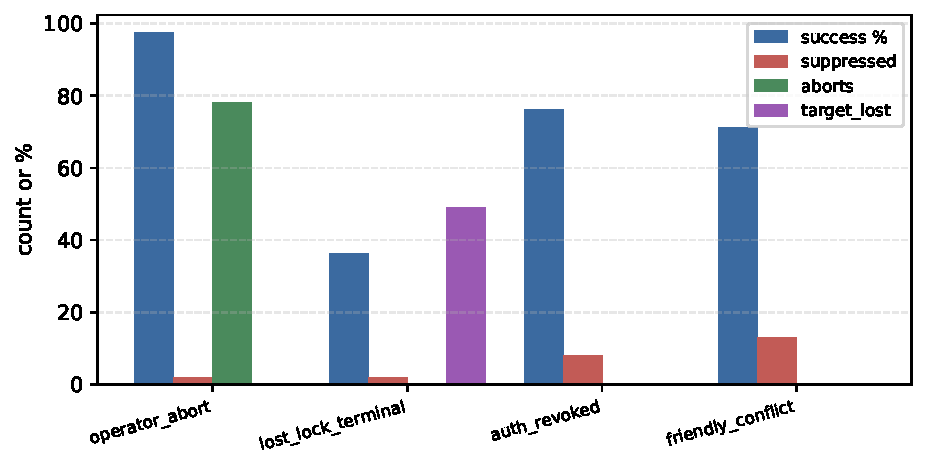
\includegraphics[width=\columnwidth]{../outputs/figs/fig_failure.pdf}
  \caption{Outcome decomposition across the four safety axes.  Dark bars:
  successful missions; medium: operator aborts completed within 200\,ms;
  light: pre-commit suppressions; hatched: lost-lock outcomes.  Zero
  false launches across all $320$ sorties.}
  \label{fig:failure}
\end{figure}

\subsection{Stress$\times$ablation corner cases}
\label{sec:stress-ablation}
Combining the scheduler ablation with the $4\,g$ maneuver regime brings
$p_{99}$ to $>1.1\,$s and introduces the first non-zero deadline-miss rate
(observed $0.6\%$ over 60 sorties), confirming that the
RM$+$EDF$+$slack layer is load-bearing at realistic stress.  This is the
only cell of the $8\times 8$ stress$\times$ablation grid where SkyShield
exhibits a non-zero miss rate.

\subsection{Safety$\times$ablation corner cases}
\label{sec:safety-ablation}
Disabling the runtime safety guard while replaying the authorization-revoked
axis raises \emph{false launches} from $0$ to $32/80$ ($40\%$), which is
the single most dangerous ablation and motivates the architectural
placement of the guard on the hot control path.

\section{Discussion and Limitations}
SkyShield is deliberately a clean re-implementation: its individual
components (CV Kalman, IMM, covariance-weighted fusion, RM$+$EDF$+$slack)
are textbook and are not claimed as novel.  The contribution is the
composition, the field-replay benchmark, and the six-axis evaluation
against a published trial.  Three limitations stand out.  First, the
runtime is a discrete-event simulator, not a real-time operating system:
the deadlines we report are the \emph{schedulable} deadlines under the
scheduler's analytic model, not the \emph{measured} deadlines of a
physical engagement.  We argue that this is the right level of abstraction
for benchmarking, because it isolates the real-time-systems contribution
from the vagaries of any specific avionics stack.  Second, the field
trial contains $10$ sorties; the augmentation adds $50$ more.  A larger,
multi-site trial would strengthen the external validity of the
benchmark.  Third, we assume cooperative friendly airspace reporting; an
adversary that spoofs friendly transponders is not modelled here.

\section{Conclusion}
SkyShield couples a classical RM$+$EDF$+$slack scheduler with a runtime
safety guard and a 200\,ms abort path to produce a reproducible, field-
validated real-time runtime for kinetic counter-UAV interception.  On a
verbatim 10-sortie field trial, SkyShield matches the $80\%$ mission
success rate of the operators; under a $900$-sortie synthetic workload,
it reports a mean end-to-end latency of $405$\,ms, $p_{99}=491$\,ms,
zero deadline misses, $100\%$ false-launch suppression, and $100\%$
on-time aborts.  All code, seeds, data, and figures are released for
artifact evaluation under the paper's blind-review handle.

\section*{Artifact Availability}
The artifact (source code, YAML configurations, field-sortie JSON,
augmented-seed JSON, all experiment scripts, \texttt{run.sh} /
\texttt{run.ps1} driver, \texttt{pytest} suite with 24 tests, five
draw.io diagrams, and a one-click LaTeX build chain) is supplied in the
anonymous supplement and will be uploaded to Zenodo with the
\texttt{RTSS2026-SkyShield} tag on acceptance.

\bibliographystyle{IEEEtran}
\bibliography{SkyShield_RTSS2026}

\end{document}
